\section*{\begin{tabular*}{\linewidth}{@{}l @{\extracolsep{\fill}} r@{}}
Nr.~9 & PIK~87/2 \\
\end{tabular*} 
}

\textsf{\textbf{Pikunda (\mbox{Sangha}; Fpl.~255)}}

\vspace{1em}

\noindent\begin{tabular}{@{}rl@{}}
\textbf{Feldarbeit:} & \textbf{03.06.--14.06.\,1987 (H. Holsten)} \\ 
\textbf{Abb.:} & \textbf{\ref{fig:PIK87-2}} \\ 
\textbf{Tab.:} & \textbf{\ref{tab:PIK87-2_Funde}}\\
\textbf{Taf.:} & \textbf{48.17--49.11} \\ 
\textbf{Lit.:} & \textbf{--} \\ 
\end{tabular} 

\begin{figure*}[tb!]
	\centering
	\begin{subfigure}[t]{\columnwidth}
		\centering
		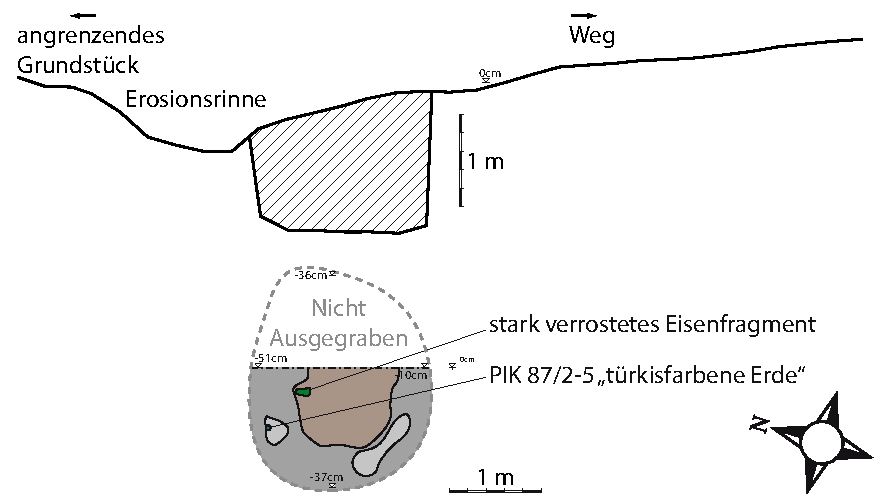
\includegraphics[width=\columnwidth]{fig/PIK87-2.pdf}
		\caption{PIK~87/2: Skizze des Befundes.}
		\label{fig:PIK87-2_PlProfSkizze}	
	\end{subfigure}\hfill
	\begin{subfigure}[t]{\columnwidth}	
		\centering
		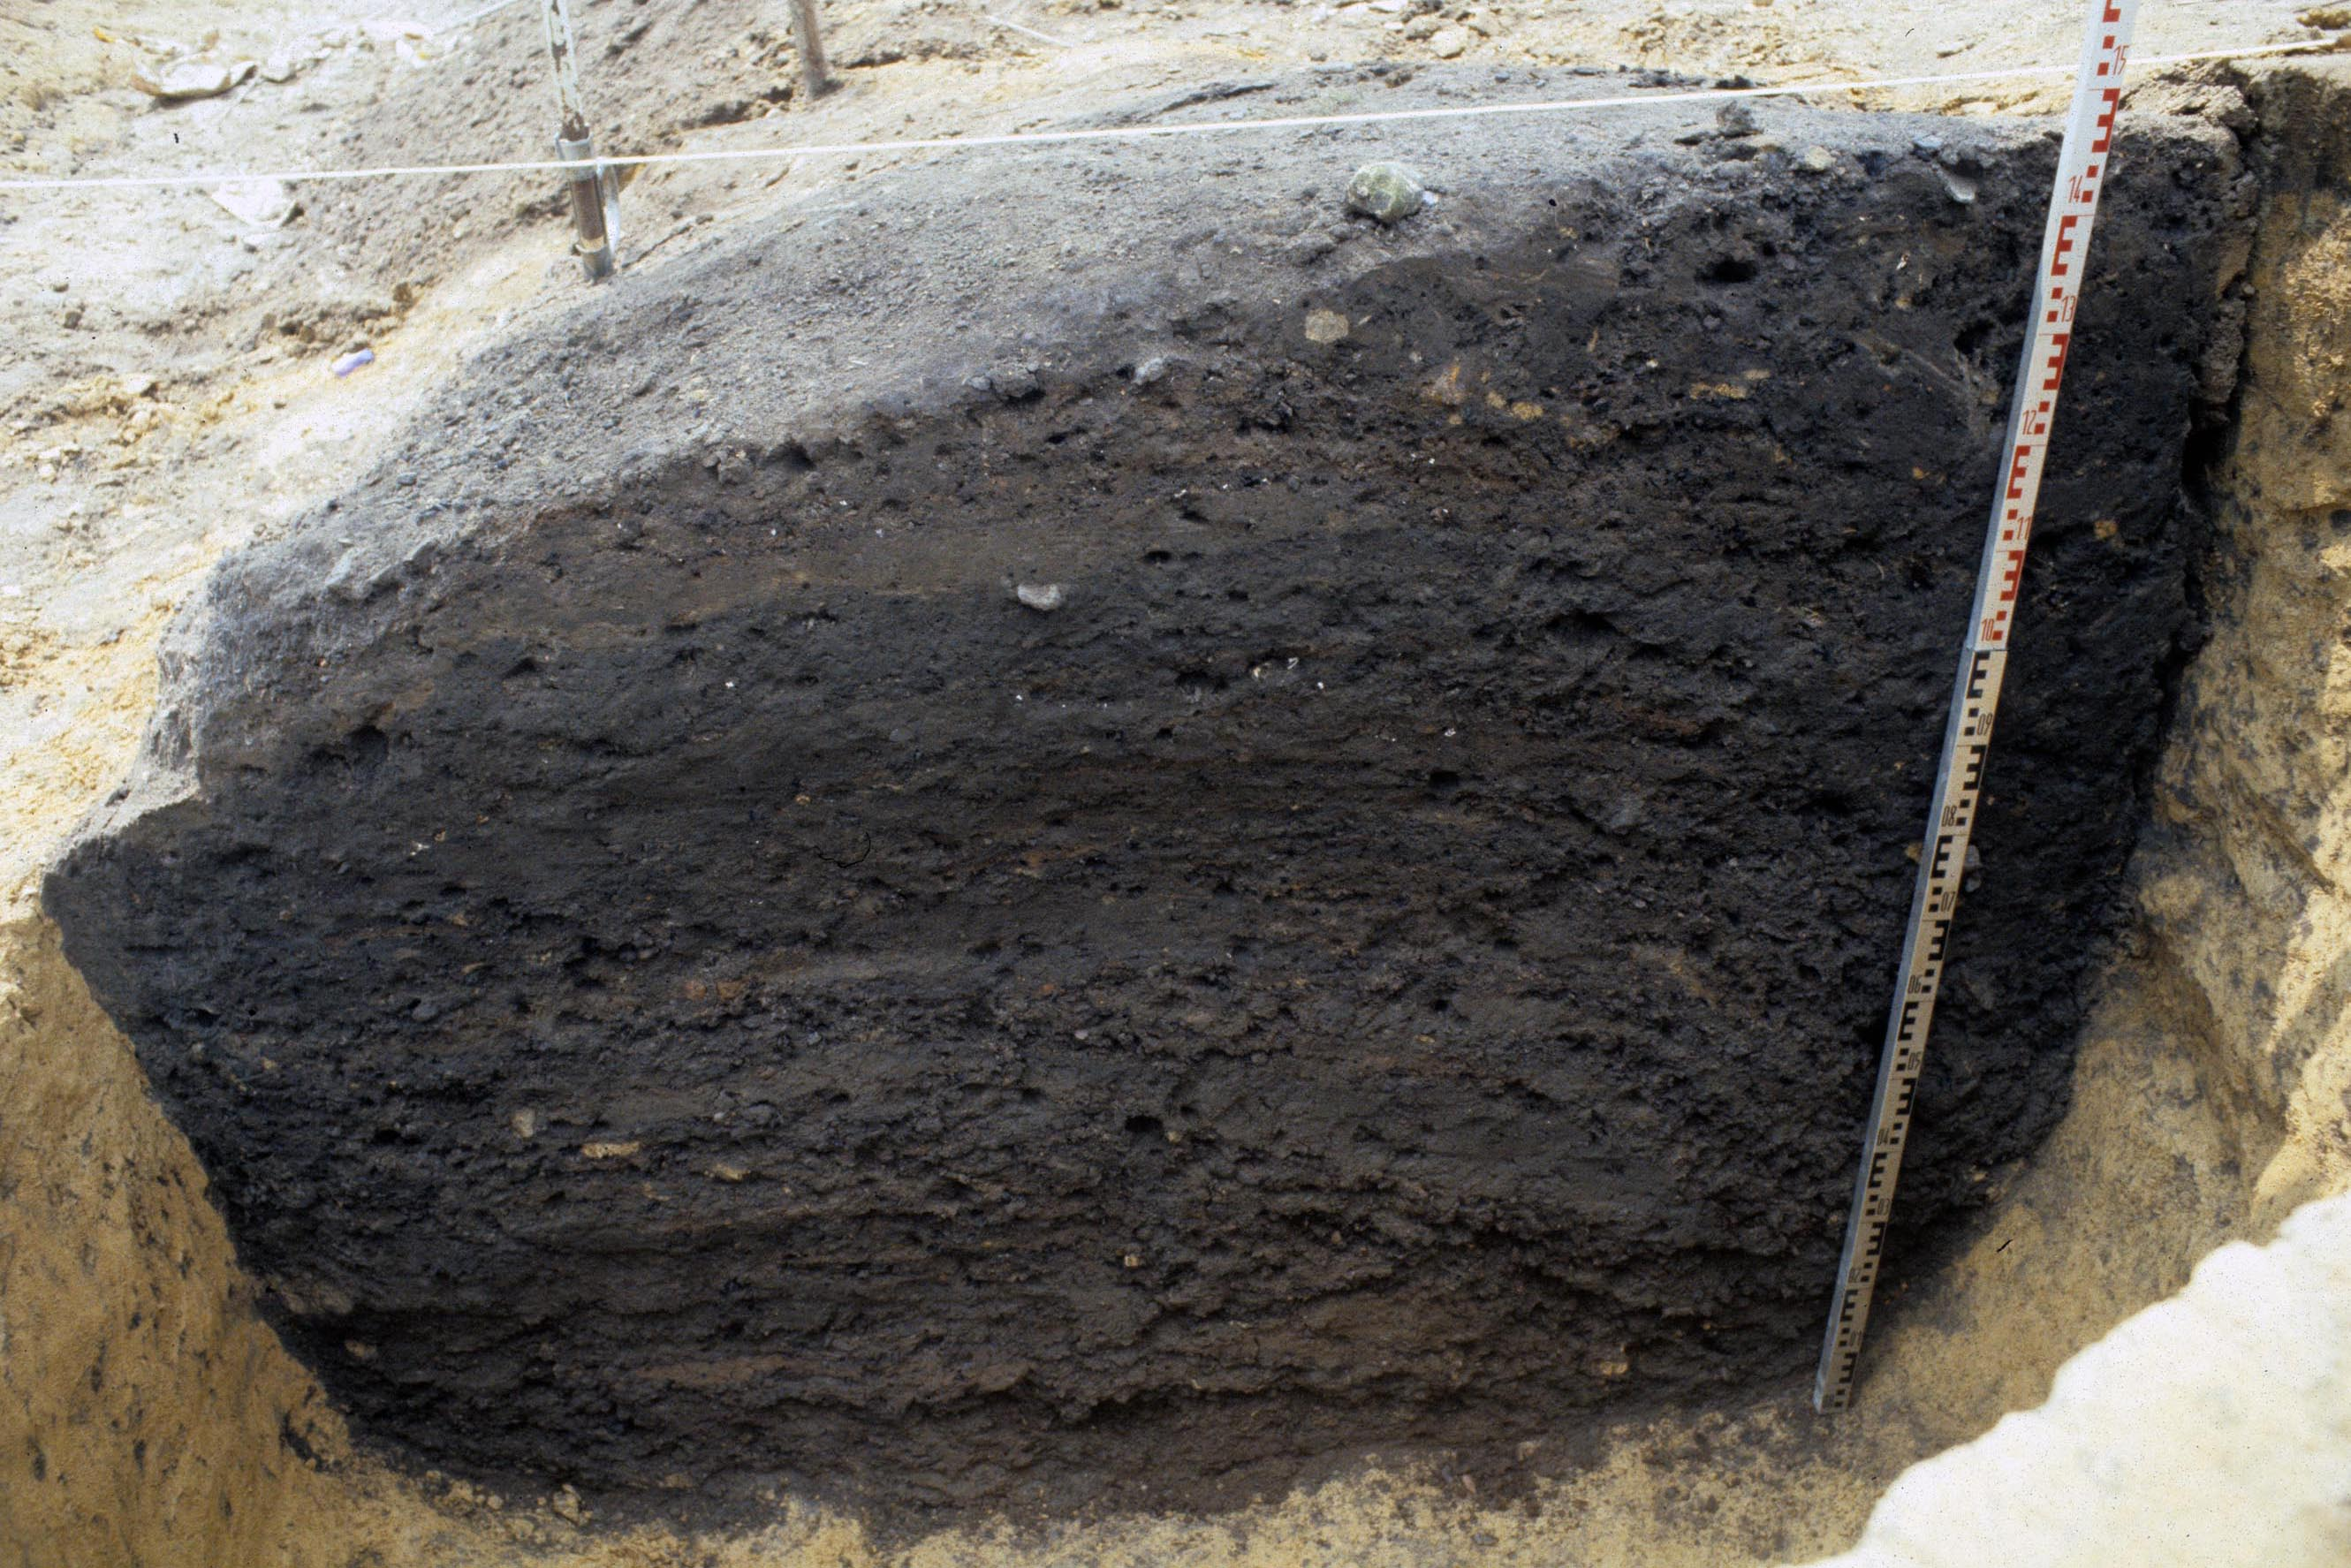
\includegraphics[width=\columnwidth]{fig/PIK87-2_Profil-H87-03-2.jpg}
		\caption{PIK~87/2: Profil (von Westen; Foto: H. Holsten, 1987).}
		\label{fig:PIK87-2_ProfilFoto}
	\end{subfigure}
	\caption{PIK~87/2: Übersicht des Befundes mit der Lage des Profils und dem Oberflächen-Nivellement entlang der Profilachse durch die Erosionsrinne sowie die Planumsskizze aus Planum 2 (T~75\,cm unter Niv.-Pkt. beziehungsweise 0,65 m unter der heutigen Oberfläche; A).}
	\label{fig:PIK87-2}
\end{figure*}

\begin{table*}[tb]
	\centering
	{\footnotesize \begin{sftabular}{@{}lrrrr@{}}
\toprule
   \textbf{Fundkategorie} &  \textbf{Anzahl} &    \textbf{\%} &  \textbf{Gewicht (kg)} &    \textbf{\%} \\
\midrule
         Botanik &       2 &   0,2 &          - &   - \\
           Eisen &       3 &   0,2 &          0,02 &   \textless\,0,1 \\
            Glas &       6 &   0,5 &          0,01 &   \textless\,0,1 \\
 gebrannter Lehm &       2 &   0,2 &          0,03 &   \textless\,0,1 \\
         Keramik &    1077 &  89,5 &         8,17 &  9,6 \\
         Keramik (1987 ausgesondert) &    - & - &         19,04 &  22,4 \\
         Knochen &      20 &   1,7 &          5,68 &  6,7 \\
         Laterit &      11 &   0,9 &          0,08 &   0,1 \\
        Ofenwand &       4 &   0,3 &          0,03 &   \textless\,0,1 \\
        Schlacke &      66 &   5,5 &          0,58 &   0,7 \\
        Schlacke (1987 ausgesondert) &      - &   - &          48,50 &   57,1 \\
        Sonstige &      11 &   0,9 &          2,74 &   3,2 \\
           Stein &       2 &   0,2 &          0,08 &   0,1 \\
\bottomrule
\end{sftabular}
}
	\caption{PIK~87/2: Anteil verschiedener Fundmaterialien.}
	\label{tab:PIK87-2_Funde}
\end{table*}

\paragraph{Grabung und Befunde}\hspace{-.5em}|\hspace{.5em}%
Etwa 30\,m östlich der Grabung PIK~87/1 (Kat.-Nr.~8) wurde ein weiterer Befund zur Hälfte ausgegraben. Es handelt sich um eine 1,5\,m tiefe, leicht ovale Grube, mit einem Durchmesser von 2--2,4\,m.\footnote{Durch eine vor der Grabung durchgeführte Sondage mit einem Pürckhauer-Bohrstock konnte eine Tiefe von 1,1--1,2\,m für den Befund ermittelt werden, wobei der Bohrkern aber sehr locker war und kaum im Bohrstock hielt. Aufgrund der Lage des Befundes in der Erosionsrinne (Abb.~\ref{fig:PIK87-2_PlProfSkizze}) und unter der Annahme, dass er einst von der ursprünglichen Oberfläche eingetieft wurde, ist davon auszugehen, dass bereits 0,2--0,8\,m der Grube erodiert waren. Das Profil durch die Grube wurde senkrecht zum Verlauf der Rinne angelegt und der Befund wurde bei der Grabung im Negativ in künstlichen Abträgen ausgenommen. Zwischen der Grubenfüllung und dem anstehenden gelben Lehm besteht eine deutlich scharfe Grenze.} Das Nord--Süd-verlaufende Profil durch die Grube PIK~87/2 zeigt eine lagige Verfüllung mit zur Grundwandung leicht abfallenden Schichtgrenzen und nur leichten Farbunterschieden zwischen den Schichten (Abb.~\ref{fig:PIK87-2_ProfilFoto}).\footnote{Da das Profil bei einem starken Regen zusammenbrach und das rezente Alter der Grube bereits im Feld erkannt wurde, wurde keine ausführliche Dokumentation angefertigt und auch die zweite Hälfte des Befundes nicht mehr untersucht.}

\paragraph{Keramik}\hspace{-.5em}|\hspace{.5em}%
Das Fundinventar aus Befund PIK~87/2 setzt sich zu etwa 30\,\% aus Keramik zusammen (Tab.~\ref{tab:PIK87-2_Funde}).\footnote{Wie im Fall des Inventars aus der Grabung PIK~87/1 (Kat.-Nr.~8) wurde auch von den Funden aus PIK~87/2 lediglich eine im Gelände gemachte Vorauswahl exportiert und 70\,\% aller Keramik im Feld verworfen. Die verworfene Keramik wurden als nicht-diagnostisch eingestuft und nach \textit{glatt}- beziehungsweise \textit{rau}-wanding differenziert gewogen. Knapp 75\,\% der aus PIK~87/2 ausgesonderten Stücke haben eine \textit{glatt} Wandung aufgewiesen.} Nahezu alle Stilgruppen, die entlang des mittleren \mbox{Sangha} beobachtet wurden (Kap.~\ref{sec:SequenzSanghaNgoko}), sind in dem stark durchmischten Inventar vertreten; von der ältesten Keramik der Region, der Pikunda-Munda-Gruppe (Kap.~\ref{sec:PKM-Gr}) bis zur rezente Ware des oberen \mbox{Sangha} und \mbox{Ngoko}, dem Mbenja-Stil (Kap.~\ref{sec:MBJ-Gr}). Einen großen Anteil nehmen rouletteverzierte Stücke ein, die das \textit{Fabric}~3 aufweisen und technisch gesehen starke Ähnlichkeiten zur Mandombe-Keramik (Kap.~\ref{sec:MDB-Gr}) aus der Grube A des Grabungsschnitts PIK~87/1 (Kat.-Nr.~8) aufweisen. Die Keramik ist stark fragmentiert. Knapp 70\,\% aller Stücke sind kleiner als 30\,$\times$\,30\,mm und Scherben größer als 120\,$\times$\,120\,mm wurden nicht beobachtet.

\paragraph{Sonstige Funde}\hspace{-.5em}|\hspace{.5em}%
Neben der Keramik bestand das Fundinventar der rezenten Grube PIK~87/2 zu knapp 60\,\% aus Schlacken, von denen etwa 84\,\% direkt im Feld verworfen wurden (Tab.~\ref{tab:PIK87-2_Funde}). Daneben fand sich im vierten Abtrag eine Glasflasche.\footnote{Die Flasche hat ein Volumen von etwa einem Liter und ist auf dem Flaschenboden mit dem Schriftzug \enquote{Halson Scotland} versehen. Die Randlippe weist auf einen Kronkorkenverschluss mit einem Durchmesser von 25,9\,mm hin.} In der Grube wurden überdies noch Fragmente von Eisenblech, Kupferdraht sowie Tierknochen und Kunstoffprodukten gefunden. Unter anderem fand sich im Bereich der Sohle eine Vielzahl von Zähnen beziehungsweise Zinken eines roten Plastikkamms. Besonders dieser Fund sowie die genannte Glasflasche legen ein deutlich junges Alter des Fundinventars nahe.

\paragraph{Datierung}\hspace{-.5em}|\hspace{.5em}%
Aufgrund der aus der Grube stammenden Funde konnte diese bereits während der Feldarbeit als rezent angesprochen werden. Eindeutig sind vor allem die Zähne eines roten Kammes aus Plastik von der Sohle der Grube sowie die eine Glasflasche aus dem vierten Abtrag. Im Lichte dieser beiden Funde sollte das Fundinventar der Grabung PIK~87/2 mit hinreichender Sicherheit in einen Zeitraum zwischen den 50er--80er Jahren des 20.~Jh. datieren.